Neste capítulo e no próximo, vamos tratar do que ocorre em $p=\pce$.
Em 2 dimensões, objeto deste capítulo, a auto-dualidade da rede $\zt$ 
permite mostrar que $\pce=1/2$ e $\theta(\pce)=0$, o que estabelece a
continuidade de $\tep$ em todo o intervalo $[0,1]$. 
Além da dualidade da rede bidimensional, outros 
ingredientes da prova são o decaimento exponencial da distribuição 
do raio de $C$ em $p<\pce$ (Teorema~\ref{teo:teo1}) e a unicidade do 
aglomerado infinito em $\tep>0$ (Teorema~\ref{teo:uni}).

Consideremos de novo, como na demonstração da Proposição~\ref{prop:trans2} 
(na página~\pageref{trans2}), a rede bidimensional dual de $\zt$, 
$$\zs=\zt+\{1/2,1/2\}.$$
$\zs$ é isomorfa a $\zt$ (por isto dizemos que $\zt$ é auto-dual).
Este fato é crucial para o que se segue. Outro fato crucial, que
já usamos na demonstração da Proposição~\ref{prop:trans2}, é a 
seguinte propriedade geométrica de $\zt$.

\vs

\bpro
\label{pro:geo}
Seja $G$ um subgrafo conexo finito de $\zt$. Existe um único circuito
$\Gamma$ de $\zs$ contendo $G$ com a propriedade de que todo elo de
$\Gamma$ cruza um elo de $\Delta G$, a fronteira de $G$ (isto é, os
elos de $\zt\backslash G$ que incidem em pelo menos um sítio de $G$).
\epro

\vs


\bte
\label{teo:2d}
Em duas dimensões,
\beqnn
\pce=1/2\quad\mbox{e}\quad\theta(\pce)=0.
\eeqnn
\ete

\vs

O Teorema~\ref{teo:2d} será provado por meio dos dois seguintes lemas.

\vs

\ble
\label{le:leb1}
Em duas dimensões,
\beqnn
\theta(1/2)=0.
\eeqnn
\ele

\vs

\bob
Este resultado tem a conseqüência imediata que em dimensão 2$$\pce\geq1/2.$$
\eob

\vs

\ble
\label{le:leb2}
Em duas dimensões,
\beqnn
\pce\leq1/2.
\eeqnn
\ele

\vs

A heurística para a validade do primeiro lema é que, se $\theta(1/2)>0$, 
então teremos um aglomerado infinito aberto em $\zt$ e 
um aglomerado infinito fechado em $\zs$. Os dois aglomerados não podem
se tocar (lembre que os elos de $\zs$ têm o mesmo status que os respectivos
elos secantes de $\zt$ --- vide a demonstração da Proposição~\ref{prop:trans2}
na página~\pageref{trans2}) e $\zt$ é pequeno demais para isto.

Para o segundo lema, a heurística é que em $p<\pce$, há apenas aglomerados
abertos finitos (ilhas) em $\zt$ num {\em mar} de elos fechados do dual.
Presumivelmente estes formam um aglomerado infinito. Logo, $1-p\geq\pce$
sempre que $p<\pce$, o que implica no resultado do lema.


\vs

\noindent{\bf Prova do Lema~\ref{le:leb1}}

O argumento, não publicado, é de Y. Zhang.
Usaremos o {\em truque da raiz quadrada} de Cox \& Durrett (já usado no
capítulo anterior na demonstração do Corolário~\ref{cor:lrc}): Se 
$$A_1,\ldots,A_m$$ forem eventos crescentes de mesma probabilidade então
$$1-\p(\cup_{i=1}^mA_i)=\p(\cap_{i=1}^mA_i^c)\geq[1-\p(A_1)]^m,$$
onde a desigualdade é FKG.
Logo
$$\p(A_1)\geq1-[1-\p(\cup_{i=1}^mA_i)]^{1/m}.$$

Suponha que 
\beq
\label{eq:abs}
\th>0.
\eeq

Seja $\aen$ o evento de que algum sítio do lado esquerdo de $\tn=[0,n]^2$
esteja num aglomerado aberto infinito de $\zt$ {\em sem} usar outros sítios de
$\tn$. Defina $\adn$, $\acn$ e $\abn$ similarmente substituindo lado esquerdo
por lado direito, lado de cima e lado de baixo, respectivamente.

Como conseqüência de~(\ref{eq:abs})
$$\ph(\mbox{existir um aglomerado aberto infinito})=1$$
de onde concluimos que
$$\ph(\aen\cup\adn\cup\acn\cup\abn)\to1$$quando $n\to\infty.$

Pelo truque da raiz quadrada,
\beq
\ph(\aun)\to1
\eeq
quando $n\to\infty$ para $u=e,d,c,b$.

Escolhamos $N$ tal que 
\beq
\label{eq:abs1}
\ph(\Anu)>7/8\quad\mbox{e}\quad\ph(\Anou)>7/8
\eeq
para $u=e,d,c,b$.

Na rede dual, sejam
$\asen$ o evento de que algum sítio do lado esquerdo de $\tsn=[0,n-1]+(1/2,1/2)$
esteja num aglomerado {\em fechado} infinito de $\zs$ {\em sem} usar outros sítios de
$\tsn$ e $\asdn$, $\ascn$ e $\asbn$ similarmente definidos substituindo lado esquerdo
por lado direito, lado de cima e lado de baixo, respectivamente.

Temos 
\beq
\label{eq:abs2}
\ph(\asnu)=\ph(\Anou)>7/8.
\eeq

Considere $$A=\ane\cap\adn\cap\asnc\cap\asnb.$$ 
Note que, em $A$, se houver apenas um
aglomerado infinito aberto em $\zt$ e apenas um aglomerado infinito fechado em $\zs$
então os caminhos abertos infinitos à esquerda e à direita de $\tne$ devem se ligar por elos
abertos por dentro
de $\tsne$ pois por fora os caminhos infinitos fechados acima e abaixo de $\tsne$ bloqueiam
a passagem. Similarmente, os caminhos infinitos fechados acima e abaixo de $\tsne$ devem se ligar
por elos fechados por dentro de $\tne$. Mas neste caso, as ligações por dentro de $\tne$ e 
$\tsne$
devem se cruzar, o que é impossível. Logo, em $A$ há dois aglomerados infinitos abertos 
disjuntos em $\zt$ ou dois aglomerados infinitos fechados disjuntos em $\zs$
(veja a Figura~\ref{fig:bid1}). Concluimos do Teorema~\ref{teo:uni} que 
\beq
\label{eq:zh}
\p(A)=0.
\eeq

\bef
%\input zh
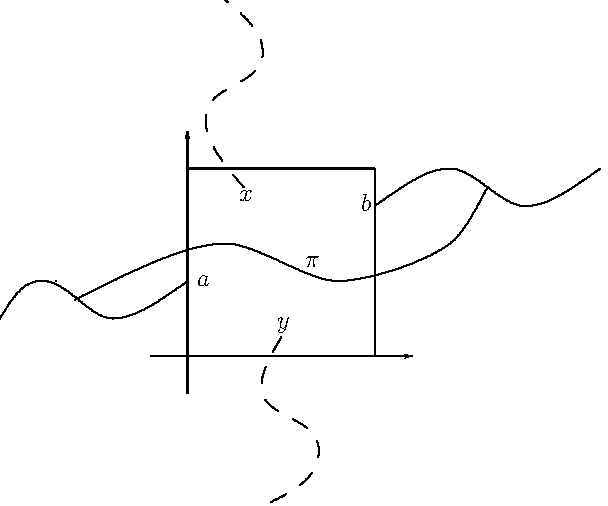
\includegraphics{zh}
\caption{Os sítios $a$ e $b$ estão em aglomerados abertos infinitos de
  $\zt\backslash T_N$ e os sítios $x$ e $y$ estão em aglomerados fechados infinitos de
  $\zs\backslash T_N^\ast$. Se houver um único aglomerado aberto infinito,
  então existe um caminho aberto $\pi$ ligando $a$ a $b$, e então os
  aglomerados infinitos fechados em $x$ e $y$ são disjuntos.}
\label{fig:bid1}
\eef

Por outro lado
\beqnn
\ph(A^c)\le\ph[(\ane)^c]+\ph[(\adn)^c]+\ph[(\asnc)^c]+\ph[(\asnb)^c]\\
\le1/2
\eeqnn
por~(\ref{eq:abs1}) e~(\ref{eq:abs2}).Logo, $\p(A)\geq1/2$, em contradição com~(\ref{eq:zh}), o que prova o lema. $\bo$





\vs





\noindent{\bf Prova do Lema~\ref{le:leb2}}

Vamos mostrar que, se $p<\pce$, então existe um aglomerado fechado infinito no
dual com probabilidade positiva, o que implica que $1-p\geq\pce$, o que por
sua vez produz o resultado do lema.

Se $p<\pce$, então do Corolário~\ref{cor:exp} temos que
\beq
\label{eq:deca}
\xip=\sum_{n=1}^\infty\p(|C|\geq n)<\infty.
\eeq
Seja $M$ um inteiro positivo e
\beqnn
\am&\!\!=&\!\!\{\mbox{Existe um caminho aberto $\pi$ em $\zt$ ligando 
algum sítio da forma}\\
&&\,\,\mbox{$(k,0)$ com $k<0$ a algum outro da forma  $(l,0)$ com
$l\geq M$ com a}\\
&&\,\,\mbox{propriedade de que todos os elos de $\pi$, a não
ser os extremos,}\\
&&\,\,\mbox{estão acima do eixo horizontal}\}
\eeqnn

\bef
%\input am
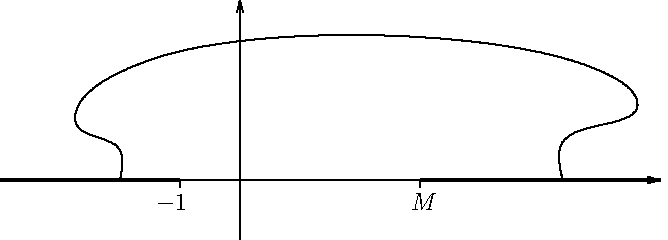
\includegraphics{am}
\caption{Um esboço do evento $\am$}
\eef

Então
\beqnn
\p(\am)\le\p\left(\bigcup_{l=M}^\infty\{(k,0)\lr(l,0)\,\,\mbox{para
    algum}\,\,k<0\}\right)\\
\le\sum_{l=M}^\infty\p((k,0)\lr(l,0)\,\,\mbox{para algum}\,\,k<0)\\
\=\sum_{l=M}^\infty\p((0,0)\lr(k-l,0)\,\,\mbox{para algum}\,\,k<0)\\
\=\sum_{l=M}^\infty\p((0,0)\lr(l+m,0)\,\,\mbox{para algum}\,\,m>0)\\
\le\sum_{l=M}^\infty\p(|C|\geq l).
\eeqnn
(\ref{eq:deca}) nos permite escolher $M$ tal que
\beq
\p(\am)\leq1/2.
\eeq

%Em $\am^c$ existe um aglomerado fechado infinito em $\zs$.

Seja agora $$L=\{(m+1/2,1/2):-1\leq m<M\}.$$ Denote por $C(L)$ o conjunto de sítios
do dual conectados a $L$ por caminhos fechados do dual.

Se $|C(L)|<\infty$, então existe um circuito aberto no dual de $\zs$, isto é
$\zt$, ao redor de $C(L)$ (pela Proposição~\ref{pro:geo}). Logo deve haver um
caminho aberto em $\zt$ ligando sítios do tipo $(k,0)$ com $k<0$ e $(l,0)$ com
$l\geq M$ inteiramente no semiplano superior. Então
\beq
\p(|C(L)|<\infty)\leq\p(\am)\leq1/2.
\eeq
Portanto $\p(|C(L)|=\infty)\geq1/2$. Mas então pelo menos um sítio de $L$ tem
que estar num aglomerado fechado infinito. De onde se conclui que
\beqnn
\p(\mbox{$0_\ast$ está num aglomerado fechado
infinito})\ge\frac{1}{M+1}\p(|C(L)|=\infty)\\
\ge\frac{1}{2(M+1)}
\eeqnn
e o lema está provado. $\bo$

\vs

A seguir apresentaremos uma outra prova do mesmo lema que tem um interessante
subproduto.

\vs


\noindent{\bf Outra prova do Lema~\ref{le:leb2}}

Considere os seguintes conjuntos de sítios
\beqnn
\Lambda_n\=\{x\in\zt:0\leq x_1\leq n+1,\,0\leq x_2\leq n\}\\
\Lambda_n^\ast\=\{x+(1/2,1/2),\,x\in\zt:0\leq x_1\leq n,\,-1\leq x_2\leq n\},
\eeqnn 
os subgrafos
\begin{eqnarray*}
S_n=\Lambda_n&\cup&\{\mbox{elos vizinhos mais próximos de $\Lambda_n$ exceto}\\
&&\quad\mbox{$(x,y)$ com $x_1=y_1=0$ ou $x_1=y_1=n+1$}\}\\
S_n^\ast=\Lambda_n^\ast&\cup&\{\mbox{elos vizinhos mais próximos de
$\Lambda_n^\ast$ exceto}\\
&&\quad\mbox{$(x,y)$ com $x_2=y_2=-1$ ou $x_2=y_2=n$}\}
\end{eqnarray*}
e os eventos
$A_n$ de que existe um caminho aberto em $S_n$ ligando seu lado esquerdo a seu lado
direito e $A_n^\ast$ de que existe um caminho fechado em $S_n^\ast$ ligando seu
lado de baixo a seu lado de cima.

\bef
%\input s5
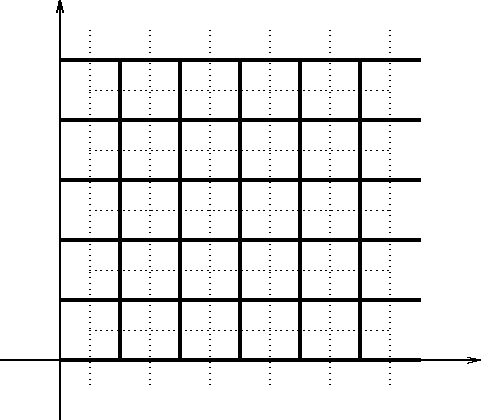
\includegraphics{s5}
\caption{$S_5$ e seu dual $S_5^\ast$}
\eef

Temos que
\beq
\label{eq:dis}
\an\cap\asn=\emptyset
\eeq
pois senão haverá um cruzamento entre caminho aberto em $\sn$ com caminho
fechado de $\ssn$, o que é impossível.

Por outro lado
\beq
\label{eq:exa}
\an\cup\asn=\Omega.
\eeq
De fato, suponha que $\an$ não ocorre. Seja $D$ o conjunto de sítios de $\sn$
alcançados da face esquerda junto com os elos ligando tais sítios.
Por uma variante da Proposição~\ref{pro:geo}, existe um caminho em
$\zs$ cruzando $\ssn$ de cima a baixo secante apenas a elos de $\sn$ contidos
na fronteira de $D$. Logo este caminho será fechado e $\asn$ ocorre (veja
Figura~\ref{fig:bid3}).

\bef
%\input du2
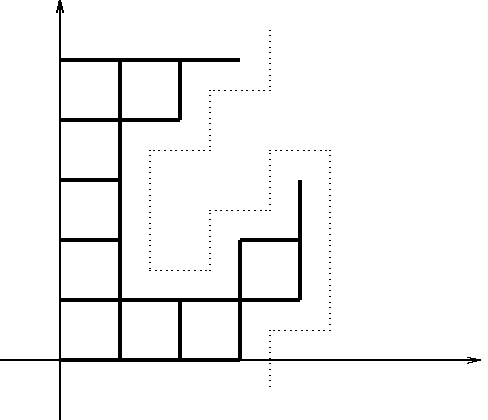
\includegraphics{du2}
\caption{Ilustração do fato de que se não há caminhos abertos atravessando 
  $\sn$ da esquerda para a
  direita, então há um caminho fechado cruzando $\ssn$ de cima para baixo.}
\label{fig:bid3}
\eef

De~(\ref{eq:dis}) e~(\ref{eq:exa})
\beq
\p(\an)+\p(\asn)=1.
\eeq
Mas $\p(\asn)=P_{1-p}(\an)$. Logo
\beq
\ph(\an)=1/2
\eeq
(para todo $n$).

Mas se $\pce>1/2$, então $\ph(\an)\to0$ quando $n\to\infty$
(por uma variante do argumento que diz que $\p(\den)\to0$
quando $n\to\infty$ se $p<\pce$ mencionado no capítulo anterior).

A contradição prova o lema. $\bo$

\vs

O subproduto interessante desta prova a que se aludiu acima é o fato
de que $\ph(A_n)=1/2$ independentemente de $n$.
Pode-se argumentar (faça-o) como para $\den$ que 
$$\p(\an)\to 0\quad\mbox{ou}\quad 1$$
quando $n\to\infty$ conforme $p<\pce$ ou $p>\pce$ respectivamente.





